\section{Non-Euclidean geometry} \label{sec:non_euclidean_geometry}

The \textit{Euclidean} geometry is based on a set of five postulates originally given by Euclid.
The postulates read as follows \cite{Weisstein-Postulates}:
\begin{enumerate}
    \item A straight line segment can be drawn joining any two points.
    \item Any straight line segment can be extended indefinitely in a straight line.
    \item Given any straight line segment, a circle can be drawn having the segment as the radius and one endpoint as the center.
    \item All right angles are congruent.
    \item Given any straight line and a point not on it, there exists one and only one straight line that passes through that point and never intersects the first line, no matter how far they are extended. \cite{Weisstein-Parallel}
\end{enumerate}
The fifth postulate, also called the \textit{parallel postulate}, has been for hundreds of years a subject of debate if it can be proven from the former four postulates.
It was discovered, however, that the negation of the parallel postulate doesn't lead to a contradiction \cite{Parallel-Postulate}.
The postulate can be negated in one of two ways.
\begin{itemize}
    \item Given any straight line and a point not on it, there exist \textbf{at least two straight lines} that pass through that point and never intersect the first line, no matter how far they are extended.
    \item Given any straight line and a point not on it, there exists \textbf{no straight line} that passes through that point and never intersects the first line; in other words, there are no parallel lines, since any two lines must intersect.
\end{itemize}

When the parallel postulate is replaced with the first statement, we obtain a new geometry, called the \textit{hyperbolic geometry}.
Similarly, replacing it with the second statement yields the \textit{spherical geometry}.
These geometries are collectively referred to as \textit{non-Euclidean geometries}.

\subsection{Analytic description}
To describe the non-Euclidean geometries analytically, we will follow the approach given by \cite{Szirmay-Kalos2022}.
This approach allows us to view the points of a 3-dimensional non-Euclidean space as a subset of the 4-dimensional \textit{embedding space}.
Since imagining the fourth dimension is not something particularly easy, we will be decreasing the dimensionality whenever we give examples.

The elliptic space can be modeled as a unit 3-sphere, \textit{embedded} in a 4-dimensional Euclidean space.
By saying that a space is embedded in another, we mean that the embedded space inherits the distance from the embedding space.
In this case, the spherical distance, given by $ds^2 = dx^2 + dy^2 + dz^2 + dw^2$ is derived from the Euclidean distance.
This is similar to how we may model the 2-dimensional elliptic space as a sphere, where lines are identified with great circles.
The inner product of two vectors $u$ and $v$ in the Euclidean space is given by
$$ \langle u, v \rangle_E  = u_xv_x + u_yv_y + u_zv_z + u_wv_w.$$
Thus, we can define that a point $p$ belongs to the elliptic geometry if
$$ \langle p, p \rangle_E = 1.$$

The model that we use for the hyperbolic geometry is the so-called \textit{hyperboloid model}.
In this model, points $p$ of the hyperbolic space satisfy the equation
$$p_x^2 + p_y^2 + p_z^2 - p_w^2 = -1,$$
with $p_w > 0$.
The set of these points creates the upper sheet of a hyperboloid, which could be visualized as shown in \autoref{fig:hyperboloid} if the embedding space was Euclidean.
\begin{figure}[h]
    \centering
    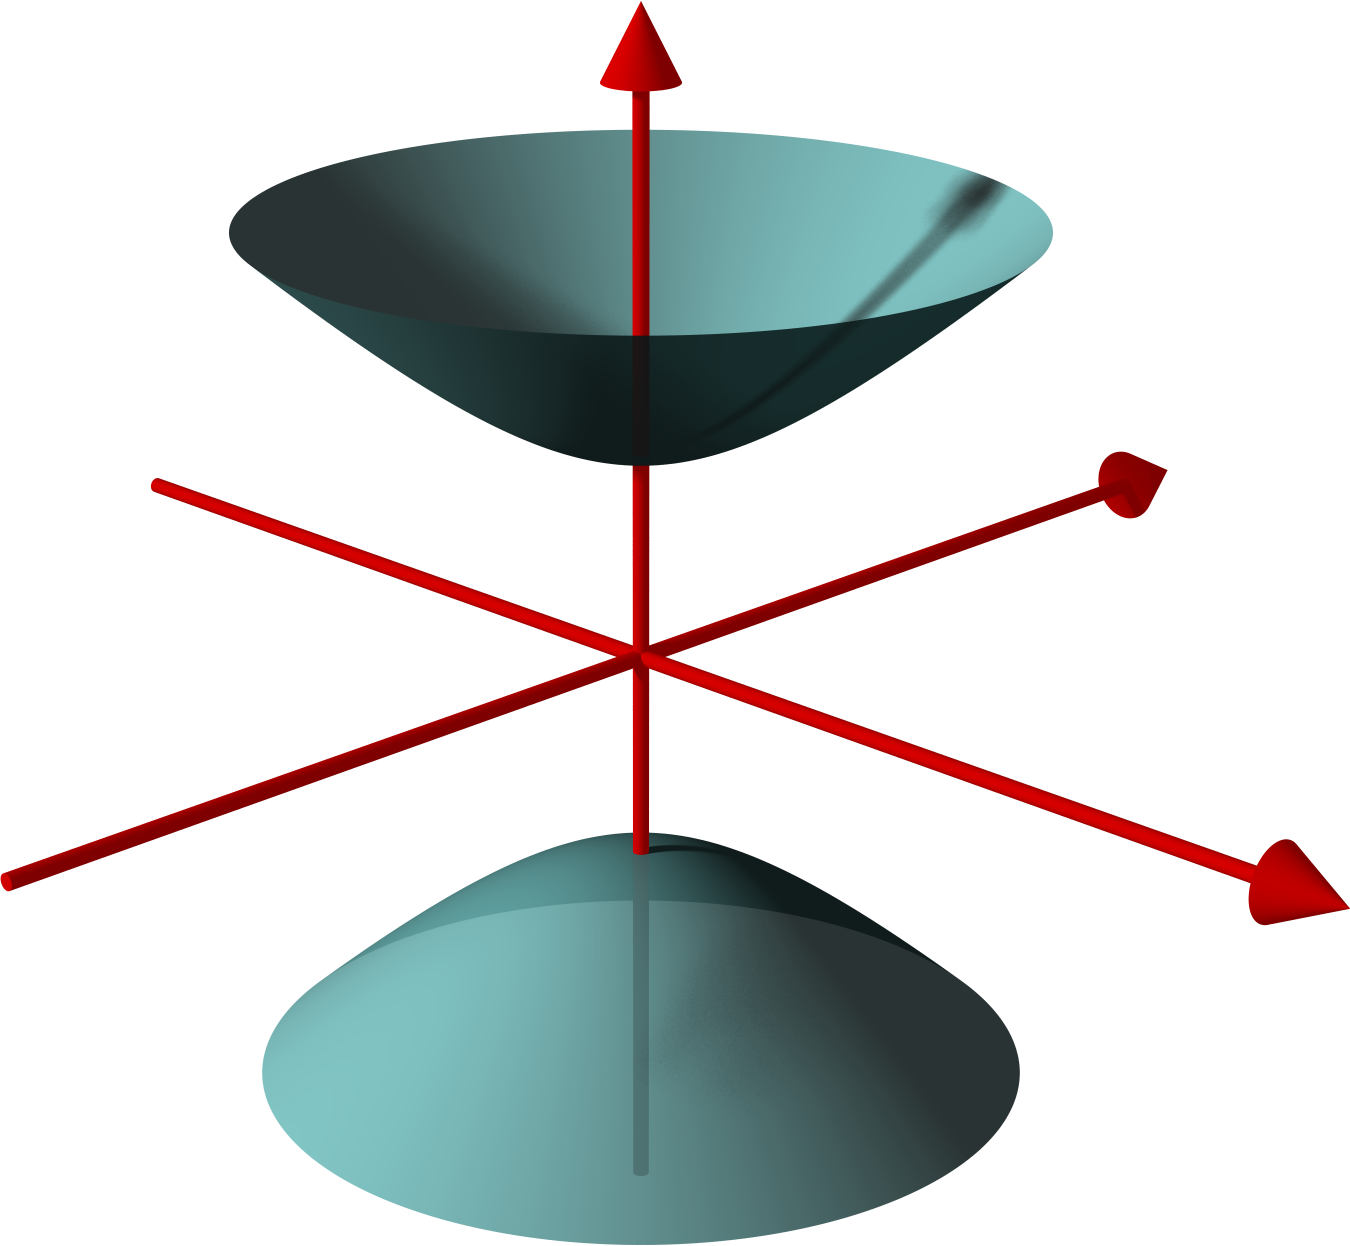
\includegraphics[width=0.4\textwidth]{chapters/theoretical_foundations/sections/non-eudlidean-spaces/resources/hyperboloid.png}
    \caption{2-dimensional hyperboloid embedded in Euclidean space}
    \label{fig:hyperboloid}
\end{figure}
However, the hyperbolic space is not embedded in the Euclidean space, but in the \textit{Minkowski space} instead.
In the Minkowski space, the inner product of vectors $u$, $v$ is given by the Lorentzian inner product:
$$\langle u, v \rangle_L = u_xv_x + u_yv_y + u_zv_z - u_wv_w.$$
Thus, the points $p$ belonging to the hyperbolic geometry satisfy the equation
$$\langle p, p \rangle_L = -1.$$
It could be interpreted that they are located on a sphere with a radius of imaginary length $\sqrt{-1}$ (and hence are equidistant from the origin).

To build a unified framework for discussing both types of geometries, we introduce the notion of \textit{sign of curvature}, $\mathcal{L}$, that attains the value $+1$ for spherical, and $-1$ for hyperbolic space.
We also define the generalized inner product
\begin{equation} \label{eq:gen-inner-prod}
    \langle u, v \rangle = u_xv_x + u_yv_y + u_zv_z + \mathcal{L}u_wv_w.
\end{equation}


\subsection{Transformations}
We will now define transformations that can be used in non-Euclidean geometries.

\subsubsection{Reflection}
A vector $v_R$ obtained from reflecting vector $v$ on vector $m$, see \autoref{fig:reflection}, can be defined as
\begin{figure}[h]
    \centering
    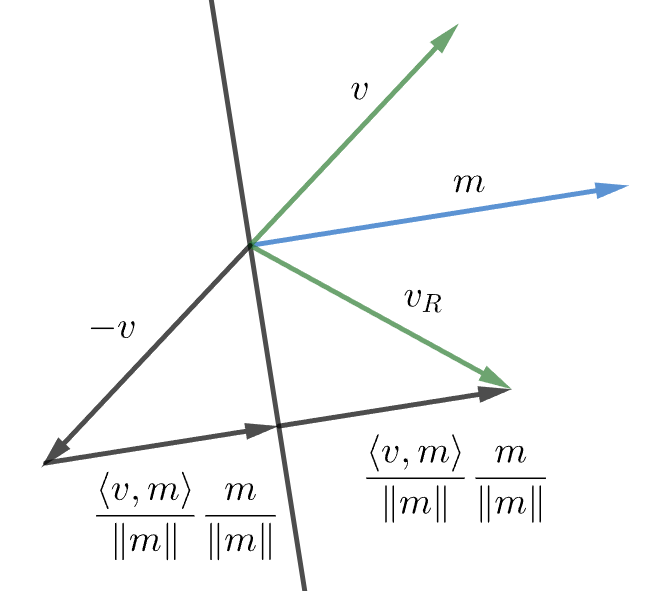
\includegraphics[width=0.4\textwidth]{chapters/theoretical_foundations/sections/non-eudlidean-spaces/resources/reflection.png}
    \caption{Reflection of $v$ on vector $m$}
    \label{fig:reflection}
\end{figure}
$$v_R = 2 \frac{\langle v, m \rangle}{\lVert m \rVert}\frac{m}{\lVert m \rVert} - v = 2\frac{\langle v, m\rangle}{\langle m,m\rangle}m - v.$$
It can be verified that this definition satisfies the intuitive conditions of a reflection:
\begin{itemize}
    \item The reflected vector $v_R$ lies in the plane spanned by $v$ and $m$,
    \item The transformation is an isometry, i.e. $\lVert u - v \rVert = \lVert u_R - v_R \rVert$.
\end{itemize}
We should also note that given a point $p$ in the geometry, i.e. satisfying $\langle p, p \rangle = \mathcal{L}$, its reflection, $p'$, is also in the geometry.

\subsubsection{Translation}
Just like in Euclidean space, we can define translation in terms of an even number of reflections.
More specifically, the translation will be defined by specifying two points: \textit{geometry origin}, $g = (0, 0, 0, 1)$ and \textit{translation target}, $q$, which is the point that the geometry origin is translated to.
Now we can define that the translation is the composition of two reflections: one on the vector $m_1 = g$ and the second one on the vector $m_2 = g + q$, which is halfway between $g$ and $q$.
Applying the first reflection to an arbitrary point $p$ gives a point
$$p' = 2 \frac{\langle p, g \rangle}{\langle g, g \rangle}g - p = 2p_w g - p,$$
and the second reflection applied to $p'$ yields a point
\begin{equation} \label{eq:translation}
    p'' = 2 \frac{\langle p', g + q \rangle}{\langle g + q, g + q \rangle}(g + q) - p'
    = 2 p_w q + p - \frac{p_w + \mathcal{L}\langle p, q \rangle}{1 + q_w}(g + q).
\end{equation}
The effect of applying translation to an arbitrary point $a$ is shown in \autoref{fig:translation}.\\
\begin{figure}[h]
    \centering
    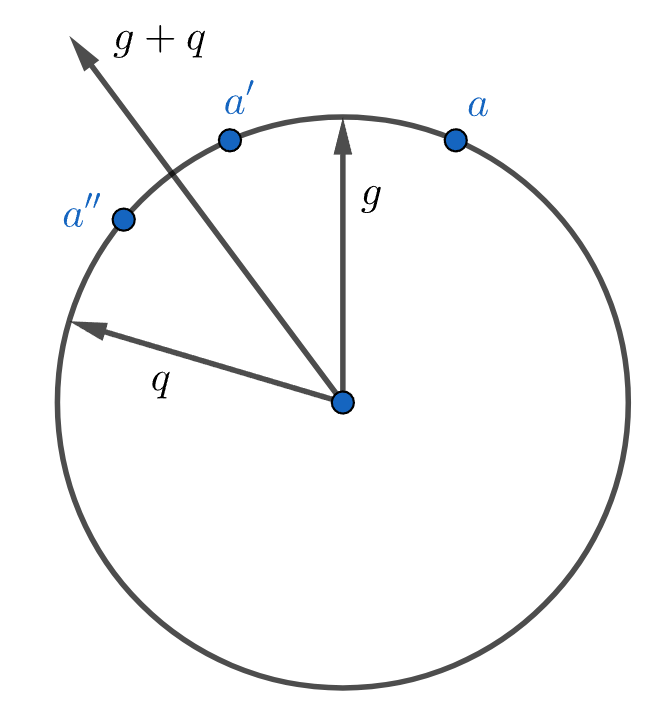
\includegraphics[width=0.4\textwidth]{chapters/theoretical_foundations/sections/non-eudlidean-spaces/resources/translation.png}
    \caption{Translation of a point $a$}
    \label{fig:translation}
\end{figure}
It can be verified that the geometry origin $g$ is indeed translated to point $g'' = q$.
We can evaluate the formula for the basis vectors $i = (1, 0, 0, 0)$, $j = (0, 1, 0, 0)$, $k = (0, 0, 1, 0)$, and $l = (0, 0, 0, 1)$ obtaining the translation matrix
\begin{equation} \label{eq:translation-matrix}
    T(q) = \begin{bmatrix}
        1 - \mathcal{L}\frac{q_x^2}{1 + q_w} & -\mathcal{L}\frac{q_x q_y}{1 + q_w}  & -\mathcal{L}\frac{q_x q_z}{1 + q_w}  & -\mathcal{L} q_x \\
        -\mathcal{L}\frac{q_y q_x}{1 + q_w}  & 1 - \mathcal{L}\frac{q_y^2}{1 + q_w} & -\mathcal{L}\frac{q_y q_z}{1 + q_w}  & -\mathcal{L} q_y \\
        -\mathcal{L}\frac{q_z q_x}{1 + q_w}  & -\mathcal{L}\frac{q_z q_y}{1 + q_w}  & 1 - \mathcal{L}\frac{q_z^2}{1 + q_w} & -\mathcal{L} q_z \\
        q_x                                  & q_y                                  & q_z                                  & q_w
    \end{bmatrix}
\end{equation}
It can be seen that the translation is an isometry since the row vectors of the matrix are orthonormal.

\subsubsection{Rotation}
It can be shown that a rotation about an axis through the origin is the same as the Euclidean rotation about the same axis \cite{Philips-Mark-Gunn1992}.

\subsubsection{Camera transformation}
% The camera transformation is defined in terms of the \textit{camera position} $e$, \textit{gaze direction} $g$, and the \textit{view-up vector} $t$.
% The camera position is a location that the camera "sees from", the gaze direction is a vector in the direction the camera is looking, and the view-up vector is a vector that points "to the sky".
% Using these vectors we can define the \textit{view space}, i.e. the camera's local coordinate system with the camera at the geometry origin and basis vectors $i'$, $j'$, and $k'$ defined as follows:
% \begin{equation*}
%     \begin{split}
%         k' = -\frac{g}{\lVert g \rVert}                    \\
%         i' = \frac{t \times k'}{\lVert t \times k' \rVert} \\
%         j' = k' \times i'
%     \end{split}
% \end{equation*}

The camera transformation allows us to describe the scene from the viewer's perspective.
The transformation is defined in terms of the \textit{eye position} $e$, and three orthonormal vectors in the tangent space of the eye:
\begin{enumerate}
    \item the right direction $i'$,
    \item the up direction $j'$, and
    \item the negative view direction $k'$.
\end{enumerate}
An example in \autoref{fig:tangent-space} shows the tangent space of the eye, with the $e$ vector marked green, $-k'$ marked blue, and $i'$ marked orange.\\
\begin{figure}[h]
    \centering
    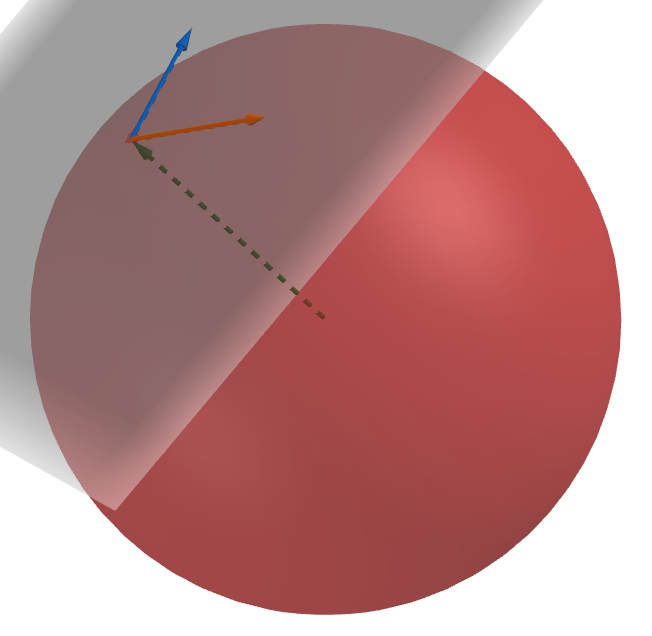
\includegraphics[width=0.4\textwidth]{chapters/theoretical_foundations/sections/non-eudlidean-spaces/resources/tangent-space.png}
    \caption{Tangent space of the camera}
    \label{fig:tangent-space}
\end{figure}
The transformation can be described by the matrix
\begin{equation} \label{eq:view-matrix}
    V =
    \begin{bmatrix}
        i'_x            & j'_x            & k'_x            & \mathcal{L}e_x \\
        i'_y            & j'_y            & k'_y            & \mathcal{L}e_y \\
        i'_z            & j'_z            & k'_z            & \mathcal{L}e_z \\
        \mathcal{L}i'_w & \mathcal{L}j'_w & \mathcal{L}l'_w & e_w
    \end{bmatrix}
\end{equation}
As the result of the transformation, the eye position is mapped to the geometry origin $g$.
Furthermore, the vectors $i'$, $j'$, and $k'$ are mapped to $i$, $j$, and $k$, respectively.

\subsubsection{Perspective transformation}
The perspective transformation is described using a projection matrix $P$.
The projection matrix we use in spherical geometry is identical to the one used in the \textit{Unity} implementation of \cite{Szirmay-Kalos2022} (see \url{https://github.com/mmagdics/noneuclideanunity}).
It is parameterized by the \textit{near plane distance} $n$, \textit{far plane distance} $f$, \textit{aspect ratio} ASP, and \textit{field of view} FOV:
\begin{equation*}
    P =
    \begin{bmatrix}
        s_x & 0   & 0  & 0  \\
        0   & s_y & 0  & 0  \\
        0   & 0   & 0  & -1 \\
        0   & 0   & -n & 0
    \end{bmatrix},
\end{equation*}
where $s_x = 2n / (r - l)$, $s_y = 2n / (t - b)$, and $r$, $l$, $t$, $b$ are defined in terms of $u = f \tan(\mathrm{FOV})$:
\begin{equation*}
    r = u \cdot \mathrm{ASP}, \,
    l = -u \cdot \mathrm{ASP}, \,
    t = u, \,
    b =  -u.
\end{equation*}
For hyperbolic and Euclidean geometries, the standard projection matrix is used.

\subsubsection*{Porting objects}
The positions of objects in the scene are specified in a 3-dimensional Euclidean space.
They are then "transported" or \textit{ported} to a non-Euclidean space of choice.
One possible mapping that could be used for this purpose is called the exponential map.
For a given point $p$ in the 3-dimensional Euclidean space with coordinates $(x, y, z)$ the mapping to elliptic geometry is given by
\begin{equation} \label{eq:elliptic-porting}
    \mathcal{P}_E(p) = (p / d \sin(d), \cos(d)),
\end{equation}
and for hyperbolic space, it is given by
\begin{equation*}
    \mathcal{P}_H(p) = (p / d \sinh(d), \cosh(d)),
\end{equation*}
where $d = \lVert p \rVert$.
The effect of porting a 1-dimensional point $p$ onto a 1-dimensional elliptic space can be seen in \autoref{fig:exp-map}.
\begin{figure}[h]
    \centering
    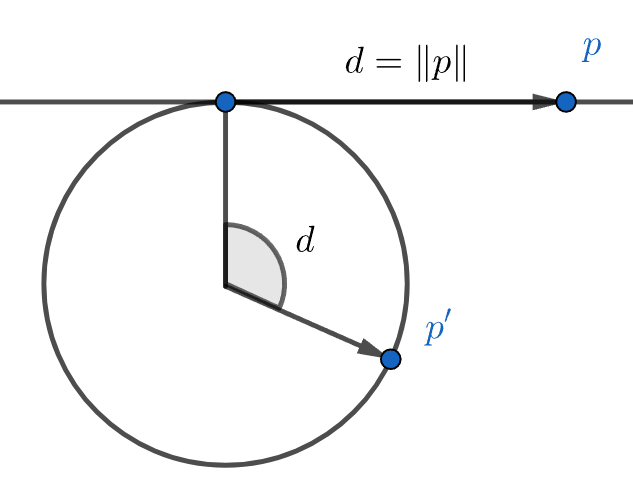
\includegraphics[width=0.4\textwidth]{chapters/theoretical_foundations/sections/non-eudlidean-spaces/resources/exp-map.png}
    \caption{Exponential map}
    \label{fig:exp-map}
\end{figure}

\subsubsection*{Porting vectors}
A vector $v$ starting at a point $p$ can be ported to non-Euclidean space by translating it to a point $\mathcal{P}(p)$.
Hence the ported vector $v'$ is given by
\begin{equation} \label{eq:porting-vector}
    v' = (v, 0) T(\mathcal{P}(p)),
\end{equation}
where $T$ is the translation matrix \ref{eq:translation-matrix}.
\subsection{Practical considerations} % based on scripts/distortions_calc.py
There are two ways we could implement placing objects in the scene:
\begin{enumerate}
    \item Port the object to non-Euclidean geometry and then use the translation given by \autoref{eq:translation},
    \item Translate the object using ordinary Euclidean translation and then port it to non-Euclidean geometry.
\end{enumerate}
The first option is undesirable, as it may significantly change the relative positions of objects in the scene.
To see why, let's consider two copies of a 2-dimensional rectangle that we will first port to the spherical geometry, and then translate using the non-Euclidean translation.
The rectangle with vertices $a = (-0.5, -0.7)$, $b = (0.5, -0.7)$, $c = (0.5, 0.5)$, $d = (-0.5, 0.5)$ is ported to spherical geometry using \autoref{eq:elliptic-porting}.
As a result, we obtain points on a unit sphere:
\begin{equation*}
    \begin{split}
         & \mathcal{P}(a) = (-0.441, -0.617, 0.652) \\
         & \mathcal{P}(b) = (0.441, -0.617, 0.652)  \\
         & \mathcal{P}(c) = (0.459, 0.459, 0.760)   \\
         & \mathcal{P}(d) = (-0.459, 0.459, 0.760)
    \end{split}
\end{equation*}
If we were to translate the first copy of the rectangle to point $t_1 = (0.5, 0.5)$ and the second copy to $t _2 = (1.5, 1.7)$ in Euclidean geometry, the two copies should meet at the point $(1, 1)$.

When we perform the translation to point $t_1$ (the corresponding translation target is obtained by porting $t_1$ using \autoref{eq:elliptic-porting}, i.e. the translation target is $q_1 = \mathcal{P}(t_1)$), we get the following vertices:
\begin{equation*}
    \begin{split}
         & T_{q_1}\mathcal{P}(a) =  (-0.014, -0.190, 0.982) \\
         & T_{q_1}\mathcal{P}(b) = (0.761, -0.296, 0.577)   \\
         & T_{q_1}\mathcal{P}(c) = (0.698, 0.698, 0.156)    \\
         & T_{q_1}\mathcal{P}(d) = (-0.110, 0.809, 0.578)
    \end{split}
\end{equation*}
The translation to $t_2$ (with $q_2 = \mathcal{P}(t_2)$) gives
\begin{equation*}
    \begin{split}
         & T_{q_2}\mathcal{P}(a) = (0.709, 0.686, 0.160)   \\
         & T_{q_2}\mathcal{P}(b) = (0.957, -0.031, -0.287) \\
         & T_{q_2}\mathcal{P}(c) = (0.141, 0.099, -0.985)  \\
         & T_{q_2}\mathcal{P}(d) = (-0.117, 0.847, -0.519)
    \end{split}
\end{equation*}
Even though we would expect the third vertex of the first copy of the rectangle to be identical to the first vertex of the second copy, there is a difference between the two.
This effect can be seen in \autoref{fig:spherical-rectangles}.
\begin{figure}[h]
    \centering
    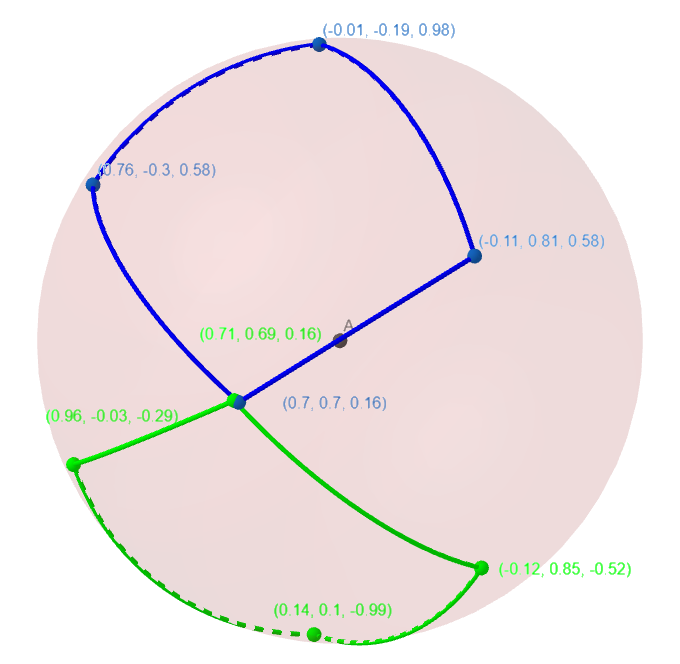
\includegraphics[width=0.6\textwidth]{chapters/theoretical_foundations/sections/non-eudlidean-spaces/resources/spherical-rectangles.png}
    \caption{Rectangles ported onto a sphere and then translated}
    \label{fig:spherical-rectangles}
\end{figure}
The effect is even more visible in the implementation. \autoref{fig:misaligned-wheel} shows how the wheels of the car get misaligned from their wheel arches.
\begin{figure}[h]
    \centering
    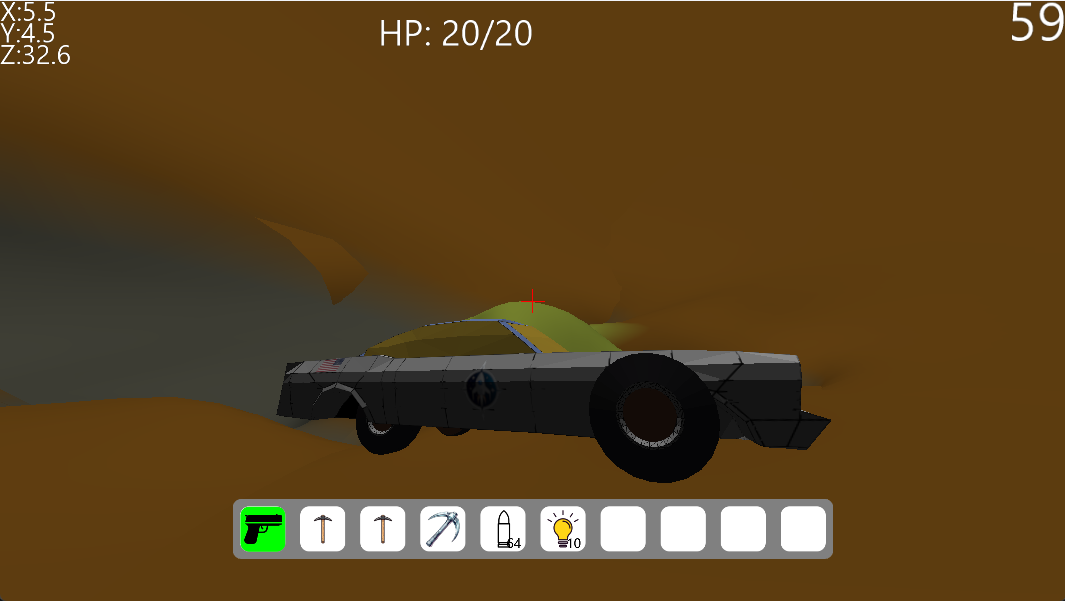
\includegraphics[width=0.6\textwidth]{chapters/theoretical_foundations/sections/non-eudlidean-spaces/resources/misaligned-wheel.png}
    \caption{Non-Euclidean translation causing a misalignment of objects}
    \label{fig:misaligned-wheel}
\end{figure}

The second option isn't unfortunately free of distortions as well.
For example, consider two identical squares of side length $0.5$.
The first one with the bottom-left corner at the point $(0,0)$ and the second one with the corresponding corner at $(0.5, 0.5)$.
After porting to spherical geometry using the \autoref{eq:elliptic-porting}, we get squares with side lengths (listed counter-clockwise starting at the bottom edge):
\begin{equation*}
    0.500, \,
    0.479, \,
    0.479, \,
    0.500
\end{equation*}
for the first square and with side lengths
\begin{equation*}
    0.480, \,
    0.425, \,
    0.425, \,
    0.480
\end{equation*}
for the second square.
The side lengths of the square have been calculated as the lengths of geodesics\footnote{This is the "great-circle distance" equal to $2 \arcsin{(c / 2)}$, where $c$ is the chord length.} between the square's vertices.
As we can see, the side lengths of the ported square are no longer equal to each other, and the distortion increases as the square is farther away from the origin.
This effect can be seen in \autoref{fig:bending-car}.
\begin{figure}[h]
    \centering
    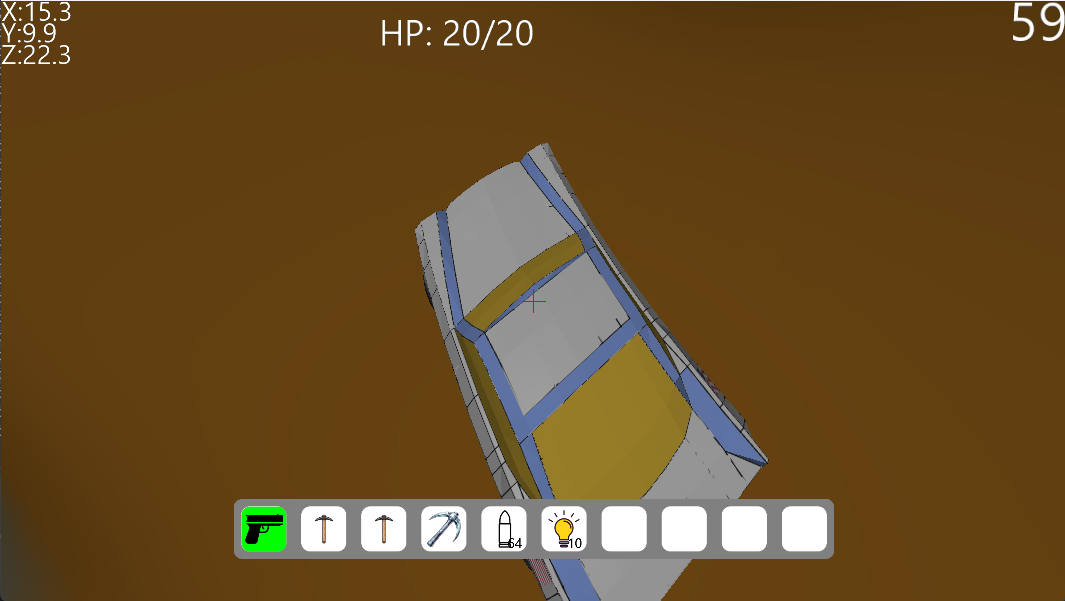
\includegraphics[width=0.6\textwidth]{chapters/theoretical_foundations/sections/non-eudlidean-spaces/resources/bending-car.png}
    \caption{Distrotions caused by porting to spherical space}
    \label{fig:bending-car}
\end{figure}

To minimize the distortions in spherical space we employed the following method.
Due to the periodic nature of the porting given by \autoref{eq:elliptic-porting}, the scene has to be confined inside a 3-dimensional ball of radius $2\pi$.
Since the distortions increase as an object is farther from the origin, we decided to split the scene into two physical regions -- balls of radius $\pi$.
Points $p$ in the first ball (centered at the origin) are mapped to spherical geometry using the mapping
\begin{equation} \label{eq:spherical-port-1}
    \mathcal{P}_{E,1}(p) = (p / \lVert p\rVert \sin(\lVert p\rVert), \cos(\lVert p\rVert))
\end{equation}
and points $p$ in the second ball (which is centered at a point $c$) using the formula
\begin{equation}\label{eq:spherical-port-2}
    \mathcal{P}_{E,2}(p) = (p' / \lVert p' \rVert \sin(\lVert p' \rVert), -\cos(\lVert p'\rVert)),
\end{equation}
where $p' = p - c$.
In the 2-dimensional case, the regions become disks with radii of length $\pi$, and the effect of using \autoref{eq:spherical-port-1} and \autoref{eq:spherical-port-2} can be visualized as "wrapping" the first disk on the upper half of a unit sphere, and "wrapping" the second one on the lower half of the sphere.

Dealing with distortions in hyperbolic space requires a more drastic approach because the scene we wished to port was potentially infinite.
The main goal was to keep the distortions as small as possible near the camera.
To achieve this, the camera position is fixed at some point close to the origin, e.g. $(0, 1, 0)$.
The movement of the camera is then simulated by moving all of the objects in the scene in the direction opposite to the camera's movement direction.
\subsection{Teleporation in spherical space} \label{sub:teleportation}
Even though splitting the scene into two regions in spherical geometry allows us to minimize distortions significantly, it introduces a wide range of other problems.
The most important one has to do with moving objects and the camera from one region to the other; we call this process \textit{teleportation}.

Teleportation is schematically shown in \autoref{fig:teleportation}.
\begin{figure}[h]
    \centering
    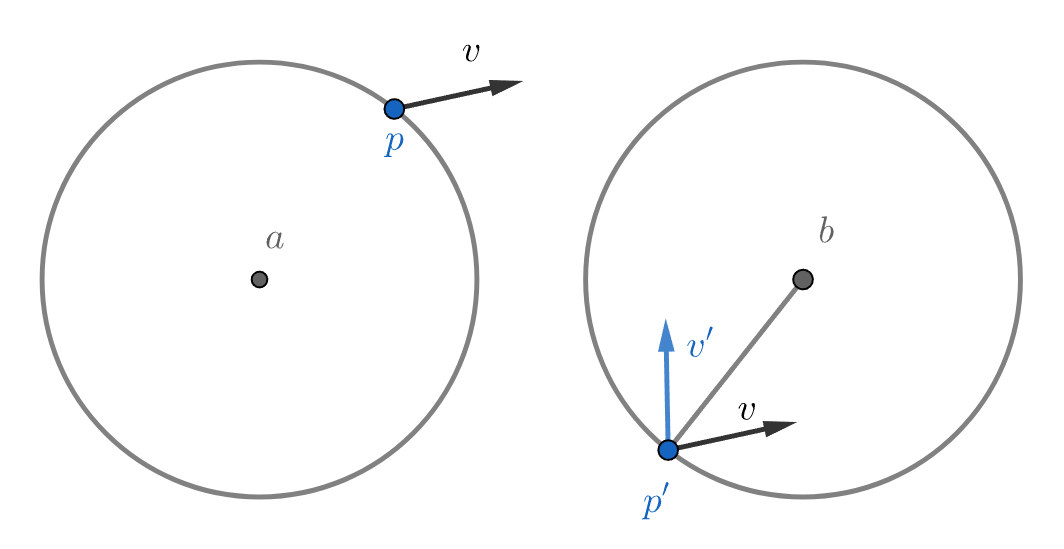
\includegraphics[width=0.6\textwidth]{chapters/theoretical_foundations/sections/non-eudlidean-spaces/resources/teleportation.png}
    \caption{Teleportation between two regions}
    \label{fig:teleportation}
\end{figure}
In this 2-dimensional example, an object leaves the first region (centered at $a$) at the point $p$ and is teleported to the second region (centered at $b$), appearing at a location given by the point $p'$:
\begin{equation*}
    p' = b + R_{xz}(p - a),
\end{equation*}
where $R_{xz}(p)$ denotes reflection of a point $p$ across the origin.
The velocity vector $v$ of the object is mapped to vector $v'$ which is the reflection of $v$ on a vector $p - a$.

The teleportation in the 3-dimensional case can be defined in a very similar manner.
There are only two differences.
The first one is that $R_{xz}(p)$ now denotes a reflection on the unit vector $\hat{y}$ (assuming positive $y$ direction coincides with the "up" direction for the scene).
The second difference is that $v'$ is now the reflection of $v$ through a plane through the origin orthogonal to $(p - a) \times \hat{y}$.

To account for the point reflection $R_{xz}$, the porting given by \autoref{eq:spherical-port-2} has to be modified by replacing $p'$ with $R_{xz}(p')$.

Setting up the view transformation in the second region also comes with its own set of challenges.
The standard way of obtaining the vectors $i'$, $j'$, and $k'$ for the view matrix \ref{eq:view-matrix} is as follows.
We first port the camera position to non-Euclidean space (in the case of the second region, we use \autoref{eq:spherical-port-2}), and then use the \autoref{eq:porting-vector} to port its right, up, and front vectors.
The problem with this approach is that the translation matrix \ref{eq:translation-matrix} is defined in terms of translating the geometry origin $g = (0, 0, 0, 1)$ and not $(0, 0, 0, -1)$.
This means that if the translation target $q$ is close to $(0, 0, 0, -1)$, $T(q)$ can map a point $p$ with $p_w < 0$ to a new point $p'$ with $p'_w > 0$ because
\begin{equation*}
    p'_w = -q_x p_x - q_y p_y - q_z p_z + q_w p_w \approx q_w p_w > 0.
\end{equation*}
The matrix isn't even defined for translation targets with $q_w = -1$.

To solve this problem, we derived a translation matrix $T_2(q)$ which we use for translations in the second region.
It is defined analogously to $T(q)$ given by \autoref{eq:translation-matrix}, but in the context of $T_2$, the translation target $q$ is the point that the point $(0, 0, 0, -1)$ is translated to.
The matrix is given by
\begin{equation}
    T_2(q) = \begin{bmatrix}
        1 - \frac{q_x^2}{1 - q_w} & -\frac{q_x q_y}{1 - q_w}  & -\frac{q_x q_z}{1 - q_w}  & q_x  \\
        -\frac{q_y q_x}{1 - q_w}  & 1 - \frac{q_y^2}{1 - q_w} & -\frac{q_y q_z}{1 - q_w}  & q_y  \\
        -\frac{q_z q_x}{1 - q_w}  & -\frac{q_z q_y}{1 - q_w}  & 1 - \frac{q_z^2}{1 - q_w} & q_z  \\
        -q_x                      & -q_y                      & -q_z                      & -q_w
    \end{bmatrix}.
\end{equation}
Using the fact that $q$ is in the spherical geometry, i.e. $\langle q, q \rangle_E = 1$, it can be verified that the row vectors of the matrix are orthonormal, thus the matrix describes an isometry.
Moreover, $T_2((0, 0, 0, -1))$ is the identity matrix as expected.